\lez{7}{02-03-2020}{}
\subsection{Indeterminazione dell'entropia}%
Cerchiamo di stimare le indeterminazioni \ldots dal punto di vista di un qualche parametro fisico del sistema.\\
Preso un sistema isolato con energia $\mathcal{E} _0$ avente un'incertezza su tale energia $\delta \mathcal{E} _0$, ci aspettiamo che la densità di stati $\rho ( \mathcal{E} ) $ sia monotona crescente nella energia \footnote{Più energia abbiamo nel sistema più abbiamo modi per distribuirla tra le varie particelle e quindi aumenta il numero di stati possibili e di conseguenza la densità di stati. Che succede se invece la densità di stati decresce con l'energia? (domanda di esame). Servirebbe un sistema con dei "Gap" tali di energia per cui, all'interno del Gap, $\rho ( \mathcal{E} ) $ diminuisce.}. \\
Se tale funzione è crescente in $\mathcal{E} $ allora possiamo scrivere:
\[
	\rho ( \mathcal{E}_{0}) \ge \frac{1}{\mathcal{E} _{0}} \int_{0}^{\mathcal{E}_{0}} \rho( \mathcal{E} ) d\mathcal{E}   
.\] 
Visto che il numero di stati nella shell spessa $\delta \mathcal{E} _{0}$ è $\rho ( \mathcal{E} _{0}) \delta \mathcal{E} _{0}$ allora l'entropia in tale regione sarà data da:
\[
	S = k\ln\left[ \rho ( \mathcal{E} _{0}) \delta \mathcal{E} _{0} \right] \ge
	k\ln \frac{\delta \mathcal{E} _{0}}{\mathcal{E} _{0}} + k\ln \int_{0}^{\mathcal{E} _{0}}\rho ( \mathcal{E} ) d\mathcal{E} 
.\] 
ci aspettiamo inoltre che
\[
	\int_{0}^{\mathcal{E} _{0}}  \rho ( \mathcal{E} ) d\mathcal{E} \ge \rho ( \mathcal{E} _{0}) \delta \mathcal{E} _{0}
.\] 
Ovvero che il volume della sfera che sta tra $0$ ed $\mathcal{E} _{0}$ sia maggiore del volumino della sola shell al bordo, per verificare questa basta prendere $\mathcal{E} _{0}$ sufficientemente grande.\\
Ci aspettiamo quindi che l'entropia sia limitata dalle precedenti disuguaglianze:
\[
	k\ln\left[ \int_{0}^{\mathcal{E} _{0}} \rho ( \mathcal{E} ) d\mathcal{E} - \ln \frac{\mathcal{E} _{0}}{\delta \mathcal{E} _{0}} \right] 
	\le S 
	\le k \ln\left[ \int_{0}^{\mathcal{E} _{0}} \rho ( \mathcal{E} ) d\mathcal{E}   \right] 
.\] 
allora l'incertezza sull'entropia dovuta all'incertezza $\delta \mathcal{E} _{0}$ sull'energia è:
\[
	\delta  S \sim k\ln \frac{\mathcal{E} _{0}}{\delta \mathcal{E} _{0}}
.\] 
Abbiamo un aspetto poco intuitivo: diminuendo l'incertezza sull'energia $\delta  \mathcal{E}_{0}$ aumenta l'incertezza sull'entropia. Questo è vero per piccole incertezze:
\[
	\frac{\mathcal{E} _{0}}{\delta  \mathcal{E} _{0}} \ll \exp\left( \frac{S}{k} \right)  
.\]
dove essenzialmente tale incertezza è un effetto di bordo. 
L'incertezza al bordo della superficie introduce una indeterminazione nel conteggio sul numero di celle che vengono attraversate dalla nostra superficie, quindi l'errore nel conteggio diventa più pesante mano a mano che restringiamo l'incertezza sull'energia. 
Siccome l'entropia è in un certo senso "l'addetta" a tale conteggio, aumenterà il suo errore restringendo lo spessore del bordo.\\
\subsection{Tempo di vita media degli stati}%
Cerchiamo di stimare $\delta \mathcal{E} _{0}$ legandola ad un parametro fisico, per far questo possiamo usufruire del principio di indeterminazione:
\[
	\delta \mathcal{E} _{0} \tau  \sim \hbar
.\] 
$\tau $ è il tempo di vita media degli stati all'interno del nostro sistema.
Quindi abbiamo dalla relazione scritta sopra:
\[
	\tau \ll \frac{\hbar}{\mathcal{E}_{0} }\exp\left( \frac{S}{k} \right) 
.\] 
Quindi il tempo di vita media degli stati non può essere infinito.\\
Tuttavia l'ultima non è una restrizione molto stringente, infatti in genere si ha che $S \gg k$, quindi l'esponenziale è un numero enorme. \\
Di conseguenza possiamo assumere che i tempi di vita degli stati termodinamici da noi considerati non siano infiniti ma comunque ragionevolmente lunghi. \\
D'altra parte noi ci aspettiamo che l'incertezza quantistica debba essere molto minore dell'incertezza termodinamica del nostro sistema, altrimenti tutte le considerazioni fatte sulla forma delle distribuzioni andrebbero completamente rivisitate (se non demolite). Quindi facendo le misure non saremo in grado di vedere $\delta \mathcal{E} _{0}$, si avrà:
\[
	\delta \mathcal{E} _{0}\ll \sqrt{\overline{\left( \Delta E \right) ^2}} = \sqrt{k C_{V}} T
.\] 
Quindi abbiamo gli estremi del tempo di vita medio $\tau $:
\[
	\frac{\hbar}{T\sqrt{k C_{V}} } \ll \tau \ll \frac{\hbar}{\mathcal{E}_{0} } \exp\left( \frac{S}{K} \right) 
.\] 
Anche quest'ultima non è particolarmente stringente, noi opereremo in sistemi aventi sempre tempi di vita così vincolati.\\
\subsection{Stati equiprobabili e teoria degli Ensamble}%
Dobbiamo rivedere adesso l'assunzione che tutti gli stati siano equalmente probabili per un sistema isolato, possiamo ottimizzarla con due assunzioni più dettagliate:
\begin{itemize}
	\item Sistema ergodico: tutti gli stati sono accessbibli nell'evoluzione temporale del sistema.
	\item Teorema di Liuville: il volume di un elemento dello spazio delle fasi si conserva nella evoluzione temporale.
\end{itemize}
Nel caso quantistico per avere gli stati equiprobabili è necessario aggiungere il \textit{Principio del bilancio dettagliato}:\\
Presi due stati $a$, $b$ la probabilità di andare da $a$ a $b$ è la stessa di andare da $b$ a $a$.
\[
	P_{a,b} = P_{b,a}
\]
Quindi il rate di passaggio da $a$ a $b$ è la stessa del passaggio opposto: 
\[
R_{a,b} = P_{a,b} W_{a} = R_{b,a}= P_{b,a} W_{b}
\]
Si può dimostrare a partire da questa che $W_{a}=W_{b}$. Infatti basta scrivere la derivata di $W_{a}$ :
\[
	\dot{W}_{a} = \sum_{b}^{} W_{b}P_{a,b} - W_{a}\sum_{b}^{} P_{a,b} = 0
.\] 
In cui il primo termne indica il rate di stati che transitano da tutti gli altri possibili ad $a$, il secondo indica quelli che invece transiscono da $a$ ad uno degli altri.\\
All'equilibrio questa derivata deve essere nulla per definizione di equilibrio stesso. Per il principio dettagliato si ha che $P_{a, b} = P_{b,a}$. di conseguenza:
\[
	0 = \sum_{b}^{} P_{a,b} ( W_{a}-W_{b}) 
.\] 
Da cui l'uguaglianza delle due $W$ risulta obbligata, a meno che il determinante di $P_{a, b}$ non sia nullo. In generale non è vero che questo determinante è nullo, quindi abbiamo la tesi.\\
Notiamo che non è detto che le $P_{a,b}$ siano tutte dello stesso ordine, tuttavia non possono nemmeno essere tutte nulle altrimenti non varrebbe più l'ergodicità. Possono esistere stati con tale quantità molto piccola, in tal caso entrare in quello stato è molto difficile ma è molto difficile anche uscirne per il principio del bilancio dettagliato.\\
In meccanica classica questi ragionamenti sono più complessi: l'ergodicità non sembra soddisfatta \footnote{Ad esempio giocando a biliardo la pallina dopo esser stata lanciata fa determinate traiettorie e si ferma, non va ad occupare l'intero tavolo da gioco.}.
Per questo in meccanica classica è stato introdotta l'idea di Ensemble: evitiamo di fare misure temporali. Così facendo il concetto di misura non è più quello di fare misure in successione temporale, bensì si fanno N copie del sistema stesso e misuriamo la probabilità facendo misure su ciascuno di questi sistemi.\\
A questo punto nelle nostre ipotesi di sistemi all'equilibrio noi abbiamo una certa probabilità di trovare il sistema di una certa energia ed il fatto di aver effettuato una misura non influnenza le successive perchè stiamo prendendo sistemi completamente equivalenti ed indipendenti.\\
Quindi nel caso classico le medie non sono medie temporali ma sono medie su campioni (copie identiche dello stesso sistema) a cui è associata una probabilità di trovare il sistema in un determinato stato.\\
In quantistica invece l'ergodicità vale quindi non ci sono problemi a fare misure temporali o "parallele".\\
Per citare la teoria dell'Ensemble possiamo riconoscere adesso che quando abbiamo usato il potenziale di Landau \footnote{Scambio di particelle ed energia con il bagno termico} abbiamo lavorato in \textit{Ensamble Gran Canonico}, con l'energia libera \footnote{Scambio di sola energia} si trattava invece di \textit{Ensamble Canonico} e quando abbiamo assunto il sistema isolata allora ci trovavamo nell' \textit{Ensamble Microcanonico}.

\subsection{Oltre il modello di gas ideale.}%
Ci sono due modi per "rovinare" il modello di gas ideale:
\begin{itemize}
	\item Facciamo cadere l'ipotesi di idealità:
	\[
		\exp\left( \frac{\mu }{kT} \right) \not\ll 1 
	.\] 
	In tal caso non funziona più il modello alla Boltzmann \footnote{Abbiamo assunto una funzione di partizione e successivamente corretto con N!} sviluppato nella \hyperref[eq:ideal_gas_approx]{Lezione 5}. \\
	Abbiamo inoltre visto che il potenziale di Landau può essere scritto in generale come:
	\[
		\Omega = \sum_{q}\Omega _{q} \implies \Omega _{q}=-kT
		\ln \left[ \sum_{n_{q}}^{} \exp\left( -\frac{n_{q}\left( \mathcal{E} _{q}-\mu  \right) }{kT} \right)  \right] 
	.\] 
	Dove ricordiamo che $q$ identifica uno stato di singola particella 
	\footnote{In un gas perfetto no interagente, dove ogni particella ha le sue $q_{x}$, $q_{y}$, $q_{z}$.} mentre $n_{q}$ è il numero di particelle che si trovano nello stato $q$.\\
	Abbiamo visto che con le approssimazioni di gas ideale possiamo riscrivere questo potenziale come nella \hyperref[eq:Landau_gas_ideale]{Lezione 4} :
	\[
		\Omega _{q} = - kT \ln \left[ 1+ \exp \left( - \frac{\mathcal{E} _{q}-\mu }{kT} \right)  \right] 
	.\]
	\[
		\overline{n_{q}} = - \frac{\delta \Omega _{q}}{\partial \mu } = \exp \left( - \frac{\mathcal{E} _{q}- \mu }{kT} \right) 	
	.\] 

\[
		\Omega _{q} = -kT \ln\left( 1+ \overline{n_{q}} \right) \sim -kT \overline{n}_{q}
	.\] 
	\[
		N = \sum_{q}^{} \overline{n}_{q} \implies PV = NkT
	.\] 
	\item Le particelle sono interagenti, abbiamo visto come si modifica il modello di gas ideale in questo caso.
\end{itemize}
Un modo pratico per uscire dalla approssimazione di gas ideale è aumentare la densità del gas: $\overline{n}_{q}$, in questo modo si rompono entrambe le approssimazioni. Possiamo notare tuttavia che la prima approssimazione a cadere nei sistemi concreti è l'approssimazione di gas perfetto: le particelle diventano interagenti \footnote{È il motivo per cui si possono trattare i liquidi classici partendo da una Z e dividendo per $N!$.}. \\
Nelle prossime lezioni invece consideriamo gas perfetti per cui non vale più la prima delle due approssimazioni. Quindi questo è il caso di gas perfetto ma non ideale \footnote{Come da definizione al paragrafo \hyperref[def:gas-ideale]{1.4.5}.}.\\
Potrebbe sembrare poco interessante studiare questo caso, tuttavia vedremo che molti sistemi (tra cui gli elettroni in un metallo) rientrano proprio in questo caso. Quest'ultimo è quindi il caso in cui fallisce la statistica di Boltzmann, è necessario trovare statistiche in grado di descrivere questi sistemi.\\

\subsection{Significato quantistico della approssimazione classica ed espressione completa di $\Omega $.}%
Anche se abbiamo tirato fuori dal formalismo la legge di stato dei gas ideali non abbiamo mai ricavato $\Omega $ dalle sue variabili indipendenti $T,V,\mu $, cerchiamo di farlo adesso con le nostre nuove conoscienze.\\
Vogliamo arrivare a scrivere $\Omega ( T, V , \mu ) $ oppure l'energia libera di Gibbs: $\Phi ( \mu , T,P) = \mu  N$, per tale scopo partiamo dal numero di particelle totale $N$ che sappiamo calcolare facilmente:
\[
	N = \sum_{q}^{} \overline{n}_{q}= \int_{0}^{\infty} \exp\left( - \frac{\mathcal{E} -\mu }{kT} \right) \rho ( \mathcal{E} ) d\mathcal{E} 
.\] 
Abbiamo trovato la densità di stati di singola particella nel caso tridimensionale:
\[
	\rho ( \mathcal{E} ) = \frac{4\pi \sqrt{2} m  ^{3 /2}}{h^3} \mathcal{E} ^{1 /2} 
.\] 
Si arriva facendo il cambio di variabile nell'integrale $x = \frac{\mathcal{E} }{kT}$ ed utilizzando la lunghezza d'onda di De Broglie $\Lambda$ ricavata nella scorsa lezione:
\[
	\Lambda = \frac{2\pi \hbar }{\sqrt{2\pi mkT} }
.\] 
Si arriva infine a:
\[
	N = \frac{V}{\Lambda ^3} \exp\left( \frac{\mu }{kT} \right)  
.\]
Possiamo invertire questo risultato per arrivare a $\mu $:
\[
	\mu = -kT \ln \frac{kT}{P\Lambda ^3} \label{eq:mu_classico}
.\] 
Quindi in conclusione a $\Phi $:
\[
	\Phi = -kT N \ln \frac{kT}{P\Lambda ^3}
.\] 
Adesso abbiamo quello che ci serve, possiamo calcolare ad esempio
\[
	V = \left.\frac{\partial \Phi }{\partial P} \right|_{T,\mu }
.\] 
Oppure possiamo calcolarci l'entropia (avendo cura di sostituire in $\Phi $ la lunghezza d'onda $\Lambda $):
\begin{align}
	S =& -\left.\frac{\partial \Phi }{\partial T} \right|_{P, \mu }=\\
		=& -Nk\ln P + \frac{5}{2}Nk \ln kT + Nk\left[ \frac{5}{2}+ \frac{3}{2}\ln \left( \frac{m}{2\pi \hbar^2} \right)  \right] =\\
		=&-Nk \ln \left( \frac{N}{V} \right) + \frac{3}{2} Nk \ln kT +Nk \left[ \frac{5}{2}+ \frac{3}{2} \ln\left( \frac{m}{2\pi \hbar ^2} \right)  \right] \\
.\end{align} 
Dove nell'ultimo passaggio abbiamo eliminato $P$ con l'equazione di stato dei gas perfetti (infatti abbiamo tolto un $N\ln kT$).\\ 
Quindi dal penultimo passaggio ricaviamo $C_{P}$, mentre dall'ultimo $C_{V}$:
\[
	C_{P} = T \left.\frac{\partial S}{\partial T} \right|_{P}= \frac{5}{2}Nk
.\] 
\[
	C_{V} = T \left.\frac{\partial S}{\partial T} \right|_{V} = \frac{3}{2} Nk
.\] 
Vista l'espressione di $\mu $ la condizione di gas perfetti si traduce allora in 
\[
	\frac{kT}{P \Lambda ^3} \gg 1
.\] 
oppure, sostituendo l'equazione dei gas perfetti:
\[
	\frac{N}{V} \Lambda ^3\ll 1 \quad \quad \text{ Approssimazione classica}
.\] 
Questa vale se la densità è molto piccola oppure se la temperatura è molto grande. Inoltre se definiamo $1 /\Lambda ^3 = d_{\text{MQ}}$ la diseguaglianza sembra affermare che la densità del gas debba essere molto minore della densità "quantistica" $d_{MQ}$. \\
Per comprendere il significato fisico della relazione sopra possiamo immaginare che l'energia media ad una certa temperatura a disposizione di una particella sia dell'ordine di $kT$, quindi il suo impulso sarà dell'ordine $\sqrt{2mkT}$.\\
L'incertezza che possiamo avere sull'impulso di una particella sarà anch'essa al massimo $\sqrt{2mkT} $, di conseguenza possiamo localizzare la funzione d'onda su dei pacchetti aventi un'incertezza dell'ordine:
\[
	 \frac{\hbar }{\sqrt{2mkT}} \sim \Lambda 
.\] 
Questo ci dice che se siamo su scale di lunghezza molto maggiore di $\Lambda $ possiamo trascurare gli effetti quantistici. Capiamo anche perchè l'ultima disuguaglianza viene detta approssimazione classica: in queste condizioni le particelle sono distanti tra loro (in media) molto più della indeterminazione quantistica che hanno sulla loro stessa posizione. In questo senso la statistica di Boltzmann viene chiamata classica.\\
Quando la disuguaglianza in questione non è più rispettata allora le particelle sono più vicine di quanto sono le loro dimensioni quantistiche (ovvero di quanto sono localizzate le loro funzioni d'onda).\\
Dal punto di vista termodinamico quando non funziona più la statistica di Boltzmann vuol dire che le particelle del gas si "accorgeranno" della loro natura quantistica, questo si traduce nell'accorgersi che le funzioni d'onda devono avere una parità ben definita a seconda dello spin.\\
Tornando alla termodinamica siamo arrivati a $\Phi $ partendo da $\Omega $, abbiamo lavorato allora nel gran canonico. In questo Ensamble abbiamo ricavato con l'algebra la funzione di stato dei gas perfetti.\\ 
Abbiamo già trovato l'equazione di stato partendo dalla Z, giudicando successivamente le particelle indistinguibili e dividendo quindi per $N!$, dobbiamo verificare che le due trattazioni sono equivalenti.\\
Rifacciamo allora il conto partendo dalla $F$ \footnote{È necessario ricordare il risultato ottenuto al termine della \hyperref[eq:F_Z]{Lezione 3} per F.}:
\[
	F = -NkT \ln \frac{V}{\Lambda ^3} + kT \ln N!
.\] 
Ma la $F$ si può calcolare anche dalla $\Phi $:
\[
	F = \Phi  - PV = -NkT \ln \frac{V}{N\Lambda ^3} - NkT
.\] 
Le due sarebero uguali se 
\[
	\ln N! \sim N \ln N-N
.\]
Visto che questa non è altro che la formula di Stirling, si ha che con $N\gg 1$ le due formulazioni danno lo stesso risultato.\\
Abbiamo fatto il conto con Z nell'ansamble canonico, poi con $\Phi $ nel gran canonico, le due trattazioni nel limite di $N\gg 1$ danno la stessa cosa perchè le fluttuazioni del numero di particelle tendono a 0 con un elevato numero di particelle.\\
Notiamo che l'entropia dell'equazione \eqref{eq:entropia1} ha una dipendenza da $-f k \ln \left( 2\pi\hbar  \right)$, con $f$ i gradi di libertà. Notiamo che questa è corretta nel caso di gas ideale, quindi in questo caso non sarà possibile utilizzarla in questa nuova statistica che stiamo costruendo.\\
Possiamo inotre notare che per i sistemi gassosi anche a basse temperature continuano a soddisfare la condizione di gas ideale, il motivo è che per ogni diminuzione della temperatura si ha una decrescita della densità per via dei passaggi di stato che inevitabilmente avvengono.\\
L'entropia sopra citata spiega molto bene questa tendenza dei gas a rimanere nello stato ideale: per un sistema qualunque tenderebbe a infinito al calare della temperatura, mentre per un gas (ad esempio l'elio) al diminire di T diminuisce anche N permettendo all'entropia di non esplodere.

\subsection{Sistemi fuori da approssimazione di gas ideale.}%
Vediamo adesso sistemi in cui le particelle sono più vicine delle loro dimensioni quantistiche. Sappiamo che le particelle in Meccanica Quantistica sono indistinguibili , di conseguenza non possiamo più correggere con $N!$ e dobbiamo utilizzare l'espressione della $\Omega$ trovata sopra.\\
Possiamo cercare di capire quali stati le particelle possono occupare.\\
Prendiamo ad esempio un caso di due particelle $( 1) $ e $( 2) $, queste saranno descritte da una funzione d'onda $\varphi_{1,2}$ che dipenderà dalle coordinate e dagli inìmpulsi delle due particelle. Se queste sono indistinguibili significa che:
\[
	\varphi ( 1,2): \left| \varphi ( 1,2)  \right| ^2 = \left| \varphi ( 2,1)  \right| ^2
.\] 
Questa ci lascia una certa libertà sulla simmetria della funzione d'onda:
\[
\varphi( 1,2) = \pm \varphi( 2,1) 
.\] 
In linea di principio potremmo assumere che ci sia una fase, tuttavia se questa fase è diversa da 0 o $\pi$ facendo un doppio scambio non si torna alla situazione iniziale, e questo non va bene per il nostro sistema \footnote{Ci sono delle particelle particolare chiamate anioni che hanno questa particolarità, le si incontrano nei corsi di fisica teorica.}.
Assumeremo da adesso che la funzione d'onda sia simmetrica o antisimmetrica scegliendo quindi soltanto le fasi $0$ e $\pi$.\\
La simmetria per scambio della funzione d'onda è connessa allo spin delle particelle di quest'ultimo:
\begin{itemize}
	\item Funzione d'onda asimmetrica: Particella con spin semi intero.
	\item Funzione d'onda simmetrica: Particella con Spin intero.
\end{itemize}
Un sistema contenente particelle con funzioni d'onda simmetriche non porta nessuna conseguenza sulla probabilità di occupazione degli stati, succedono cose strane invece per sistemi contenenti particelle con funzione d'onda antisimmetriche.
\paragraph{Distribuzione di Fermi-Dirac e Fermioni}%
Supponendo che le particelle si trovino in due stati $A$ e $B$ e che la funzione d'onda sia antisimmetrica allora si ha che:
\[
	\varphi_{A,B} \propto \Phi _{a}( 1) \Phi _{b}( 2) - \Phi _{a}( 2) \Phi _{b}( 1) 
.\] 
Abbiamo così una funzione antisimmetrica, tuttavia se adesso prendiamo i due stati $A$ e $B$ uguali si ha che $\varphi = 0$. Quindi non di può avere più di una particella in ogni singolo stato. \\
Nota: Per rendere asimmetrica una funzione d'onda ad esempio con tre particelle si procede così:
 \[
	 \Phi _{a}( 1) \Phi _{b }( 2) \Phi _{c}( 3)  - \Phi _{a}( 2) \Phi _{b }( 1) \Phi _{c}( 3) +   \Phi _{a}( 2) \Phi _{b }( 3) \Phi _{c}( 1)
.\] 
Quindi se volessimo calcolare la $\Omega _{q}$ dello stato $q$:
\[
	\Omega _{q}= -kT \ln \sum_{n_{q}}^{} \exp\left( - \frac{n_{q}\left( \mathcal{E} _{q}- \mu  \right) }{kT} \right) \label{eq:Landau-Generic}
.\] 
Non si deve più sommare su tutte le possibili $n_{q}$, la somma si ferma al primo termine poichè al massimo una sola particella può stare in uno stato:
\[
	\Omega _{q} = - k T \ln \left[ 1 + \exp\left( \frac{\mu - \mathcal{E} _{q}}{kT} \right)  \right] 
.\] 
Questa è la stessa che abbiamo trovato nel modello dei gas ideali approssimando (Sezione \ref{sec:Boltzmann_distrib}), solo che questa non è una approssimazione: è esatta! Inoltre trovoata la $\Omega _{q}$ siamo costretti a fermarci: non è più vero che $\overline{n_{q}}\ll 1$ come invece abbiamo imposto nella \ref{eq:Landau_Boltzmann}. \\
Troviamo allora il numero medio di particelle che stanno in ciascun stato di singola particella $\overline{n}_{q}$ tramite la relazione del potenziale di Landau:
\[
	\overline{n}_{q} = - \frac{\partial \Omega _{q}}{\partial \mu } =
	\frac{\exp\left( \frac{\mu - \mathcal{E} _{q}}{kT} \right)  }{1 + \exp\left( \frac{\mu - \mathcal{E} _{q}}{kT} \right) } = \frac{1}{\exp\left( \frac{\mathcal{E}_{q}-\mu }{kT} \right) +1}
.\] 
Dalla funzione notiamo che $\overline{n_{q}}<1$, questo è coerente con quanto detto in precedenza su le particelle aventi funzione d'onda asimmetrica (quindi spin semintero): più di una particella in un singolo stato non ci può stare.
Abbiamo ricavato una prima importante distibuzione:

\begin{defn}[Distribuzione di Fermi-Dirac]{def:Distribuzione di Fermi-Dirac}
	Il numero medio di particelle negli stati di singola particella $q$ per un gas di fermioni è dato da:
	\[
		\overline{n}_{q} = \frac{1}{\exp\left( \frac{\mathcal{E} _{q}-\mu}{kT} \right) +1}
	.\] 
	L'energia $\mu$ a temperatura $T = 0$ è detta energia di Fermi $\mathcal{E}_{F}$.
\end{defn}
La forma di questa funzione è la seguente:
\begin{figure}[H]
	\centering
	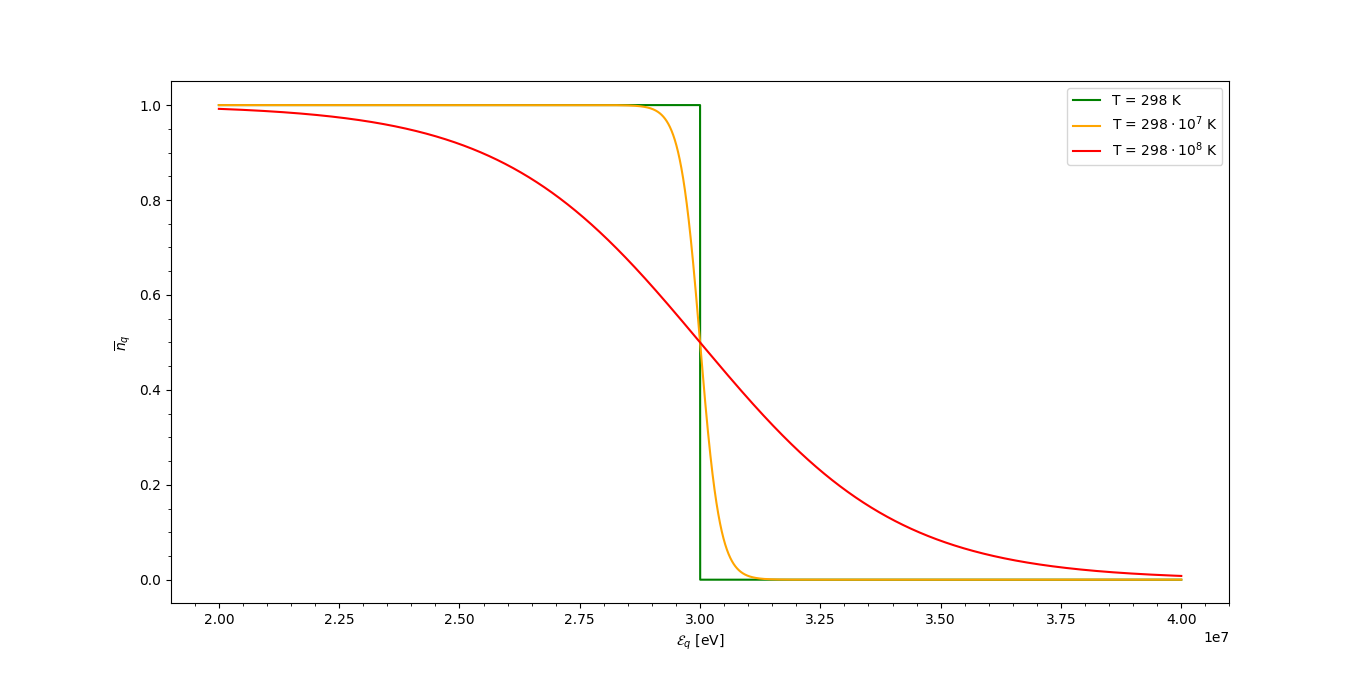
\includegraphics[width=0.9\textwidth]{figures/fermi_dirac.png}
	\caption{\scriptsize Distribuzione di fermi dirac realizzata in python per varie temperature e per $\mu = 30$ MeV, tipico dei gas di elettroni atomici.}
	\label{fig:figures-fermi_dirac-png}
\end{figure}
\noindent
Notiamo come a basse temperature ($kT \ll \mu$) la funzione sia praticamente un gradino che crolla sulla $\mu$, in questo caso lo smusso del gradino è proprio dell'ordine di $kT$.\\
Di fatto a $T\approx 0$ si ha che le particelle si dispongono in modo da minimizzare l'energia (andranno nei livelli energetici più bassi), quindi se voglio aggiungere una particella al sistema dovrò aggiungerla con una energia maggiore di quella delle particelle già presenti perchè tutti gli stati con energia inferiore sono occupati. Quindi per aggiungere questa particella dorvò dare una energia di almento $\mu$. L'energia $\mu = \mathcal{E}_{0}$ a temperatura nulla rappresenta di fatto la linea di demarcazione tra gli stati occupati e gli stati vuoti.\\
Questo ci da informazioni sul fatto che, se $T \to 0$, il potenziale chimico non potrà essere negativo perchè in tal caso il numero di particelle medio per ogni stato è nullo, quindi sparirebbero tutte le particelle dal sistema.\\
Ricordiamo che stiamo sempre considerando il sistema all'equilibrio con un bagno termico in cui abbiamo tenuto $\mu $ costante \footnote{Questo a livello fisico significa poter variare il numero di particelle al variare della temperatura, infatti il potenziale chimico è la variazione dell'energia del sistema rispetto al numero di particelle: per mantenerlo costante al variare dell'energia serve che cambi il numero di particelle.}, variare la temperatura significa variare la temperatura di questo "universo".\\
Spesso nei sistemi veri dobbiamo tener di conto che il numero di particelle del sistema in considerazione (bagno termico escluso) potrebbe essere fissato. In questo caso la legge resta valida però $\mu$ non è più fissato.\\
In questo caso possiamo aspettarci che esista una temperatura oltre il quale torniamo nella approssimazione classica di Boltzmann quindi il potenziale chimico dovrà tornare negativo e molto grande. \\
Possiamo dire anche qualcosa in più sul numero di particelle totali per questa distribuzione:
\[
	N = \sum_{q}^{} \overline{n}_{q} = \int_{0}^{\infty} \rho ( \mathcal{E} ) \cdot \frac{1}{\exp\left( \frac{\mathcal{E} -\mu }{kT} + 1 \right) } d\mathcal{E} 
.\] 
\paragraph{Distribuzione di Bose-Einstein e Bosoni}%
Nel caso in cui le particelle abbiano spin intero non abbiamo più nesuna condizione sulla occupazione degli stati, quindi non possiamo più tagliare al secondo termine nella sommatoria \ref{eq:Landau-Generic}, possiamo invece fare un cambio di variabile:
\begin{align}
	x = \exp\left( \frac{\mu -\mathcal{E} }{kT} \right) \implies
	\Omega _{q} = -kT \ln \left[ \sum_{n_{q}}^{} x^{n_{q}} \right] 
.\end{align}
Sappiamo che per non esplodere questa serie geometrica necessita che $x<1$, quindi che $\mu < \mathcal{E} _{q}$.
L'ultima disuguaglianza deve essere vera per tutti gli $\mathcal{E}_{q}$, quindi nel caso peggiore per lo stato con $\mathcal{E} = 0$, abbiamo allora una condizione sul potenziale chimico per la convergenza della serie:
\[
	\mu < 0
.\] 
Questo ci va bene perchè è conforme con quanto detto per il regime classico, dove anche in quel caso $\mu$ doveva essere negativo (in tal caso c'era una ulteriore condizione: doveva essere molto negativo).\\
Visto che la serie per $\Omega _{q}$ è geometrica si ha che la somma vale:
 \[
	 \Omega _{q} = kT \ln\left( 1-\exp\left( -\frac{\mathcal{E} _{q}-\mu }{kT} \right)  \right) 
.\] 
Quindi ci ricaviamo il numero medio di particelle: 
\[
	\overline{n}_{q} = - \frac{\partial \Omega _{q}}{\partial \mu } = \frac{1}{\exp\left( \frac{\mathcal{E} _{q}- \mu }{kT} \right)-1 }
.\] 
Abbiamo ottenuto una distribuzione simile alla Fermi-Dirac con un segno diverso, quel segno cambia pesantemente la forma della distribuzione che chiameremo:
\begin{defn}[Distribuzione di Bose-Einstein]{def:Distribuzione di Bose-Einstein}
	Il numero medio di particelle negli stati di singola particella $q$ per un gas di bosoni è dato da:
	\[
		\overline{n}_{q} = \frac{1}{\exp\left( \frac{\mathcal{E} _{q}-\mu}{kT} \right) - 1}
	.\]
\end{defn}
Graficamente la distribuzione con $\mu$ fissato è così fatta:
\begin{figure}[H]
	\centering
	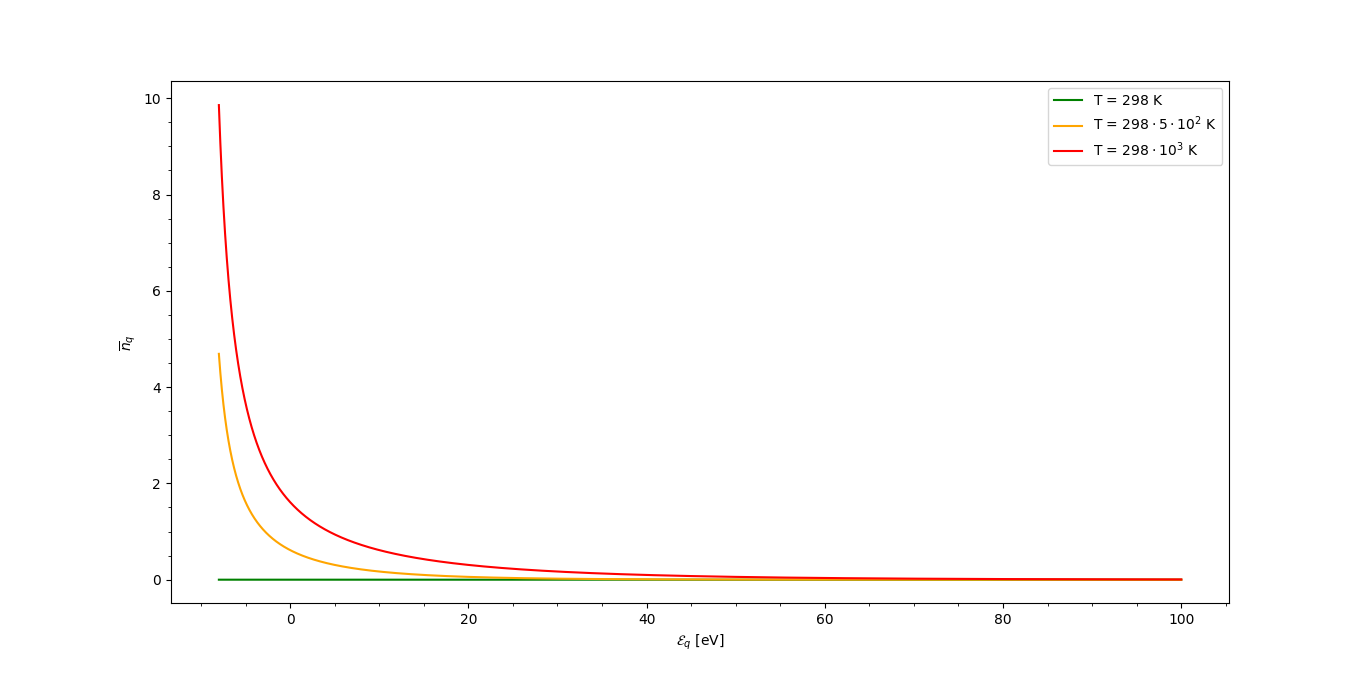
\includegraphics[width=0.95\textwidth]{figures/bose_einstein.png}
	\caption{\scriptsize Distribuzione di Bose-Einstein per $\mu = -10$ eV fissato.}
	\label{fig:figures-bose_einstein-png}
\end{figure}
\noindent
Questa è la Bose Einstein, e le particelle di spin intero sono perciò detti Bosone.\\
Tenere $\mu $ fissato anche in questo caso significa tenere libero il numero di particelle del sistema che quindi potrà essere scambiato con il bagno termico. La conseguenza che ne risulta dal grafico è che al diminuire della temperatura le particelle tenderanno a scappare dal sistema per spalmarsi in tutto l'universo (nei livelli di energia più bassa disponibili).\\
Nel limite classico entrambe le distribuzioni tornano al limite di Boltzmann classico.
